\section{METODOLOGIA EXPERIMENTAL}

\subsection{MATERIAIS}
Para o desenvolvimento das atividades propostas pelo experimento foi utilizado o software de simula��o OrCAD.

\subsection{M�TODOS}
A pr�tica no laborat�rio consistiu no desenho e simula��o deste circuito:
	\begin{figure}[H]
		\centering
		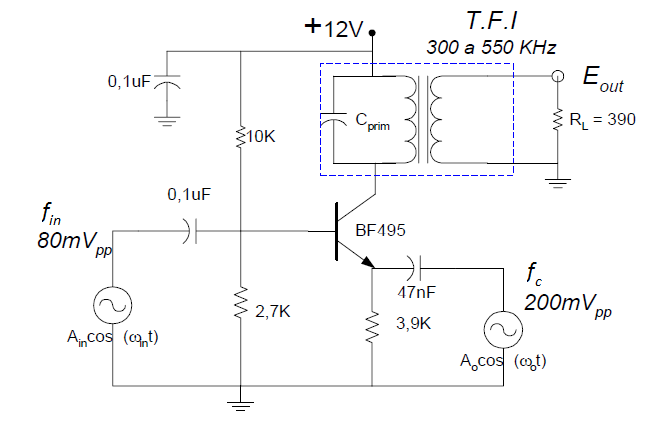
\includegraphics[scale=.6]{imagens/cir1.png}
		\caption{Circuito 1}
	\end{figure}

\begin{itemize}
	\item[$\bullet$] Atividade 1 - Determina��o do filtro
	\item[$\bullet$] Atividade 2 - Down-Converter e Up-Converter
	\item[$\bullet$] Atividade 3 - Uso de um amplificador seguidor de emissor
\end{itemize}

\subsubsection{Determina��o do filtro}
Foi necess�rio calcular os valores dos componentes que n�o est�o determinados: o indutor(transformador) e capacitor ligados ao coletor do transistor. Estes elementos formam um filtro passa faixas cuja frequ�ncia de oscila��o ditar� a frequ�ncia do sinal de sa�da. O transformador utilizado tem uma rela��o de espiras de 8:1, ou seja, o indutor do secund�rio deve ser 64 vezes menor do que o do prim�rio. 

